%==============================================================================
%  DSCI 6000 小组作业 2 —— 贝叶斯统计推断（广告点击率分析）
%  最终版正式报告  ·  编译方式：xelatex report.tex （需运行两次以生成目录）
%  模板：ctexart + 与封面 academic_cover_v2.pdf 一致的配色/版式
%==============================================================================
\documentclass[12pt,a4paper,UTF8,fontset=none]{ctexart}

%------------------------------- 页面与字体 -----------------------------------
\usepackage[a4paper,top=2.6cm,bottom=2.4cm,left=2.5cm,right=2.5cm,
            headheight=23pt,footskip=1.1cm]{geometry}

\usepackage[table,dvipsnames]{xcolor}
\usepackage{amsmath,amssymb}
\usepackage{graphicx}
\usepackage{float}
\usepackage{booktabs}
\usepackage{tabularx}
\usepackage{array}
\usepackage{enumitem}
\usepackage{fancyhdr}
\usepackage{caption}
\usepackage{pdfpages}
\usepackage{listings}
\usepackage[listings,breakable,skins]{tcolorbox}
\usepackage[colorlinks=true,unicode]{hyperref}
\usepackage{xurl}
\usepackage{etoolbox}
\usepackage{needspace}
\usepackage[titles]{tocloft}

% 中文字体：Noto Serif/Sans CJK SC（与封面一致的宋/黑搭配）
\setCJKmainfont{Noto Serif CJK SC}[
  BoldFont      = Noto Serif CJK SC Bold,
  ItalicFont    = Noto Serif CJK SC,
  BoldItalicFont= Noto Serif CJK SC Bold]
\setCJKsansfont{Noto Sans CJK SC}[BoldFont = Noto Sans CJK SC Bold]
\setCJKmonofont{Noto Sans Mono CJK SC}[BoldFont = Noto Sans Mono CJK SC Bold]
% 西文字体
\setmainfont{TeX Gyre Termes}
\setsansfont{TeX Gyre Heros}
\setmonofont{DejaVu Sans Mono}[Scale=MatchLowercase]

%------------------------------- 配色（取自封面） ------------------------------
\definecolor{navy}{HTML}{1A365D}      % 深蓝：标题
\definecolor{accent}{HTML}{2B6CB0}    % 亮蓝：强调、链接、装饰条
\definecolor{softbg}{HTML}{F7FAFC}    % 极浅底：表格斑马纹 / 代码底
\definecolor{linegray}{HTML}{CBD5E0}  % 中灰：分隔线
\definecolor{bordergray}{HTML}{E2E8F0}% 浅灰：边框
\definecolor{inkgray}{HTML}{4A5568}   % 次要文字
\definecolor{codekw}{HTML}{2B6CB0}
\definecolor{codestr}{HTML}{2F855A}
\definecolor{codecmt}{HTML}{718096}

\hypersetup{
  linkcolor  = navy,
  urlcolor   = accent,
  citecolor  = accent,
  pdftitle   = {DSCI 6000 小组作业 2：贝叶斯统计推断 —— 广告点击率分析},
  pdfsubject = {Bayesian Statistical Inference / Beta-Binomial Conjugate Analysis},
  pdfauthor  = {Team 12：王金波、何漪雯、李敏、丁玲、刘海龙},
  pdfkeywords= {Bayesian, Beta prior, Binomial likelihood, Posterior, Credible Interval, CTR},
  bookmarksnumbered = true,
}

%------------------------------- 标题样式 -------------------------------------
% 与封面呼应：一级标题深蓝无衬线 + 通栏蓝色细线；二级标题左侧蓝色竖条
\newcommand{\headbar}{\textcolor{accent}{\rule[-0.12em]{2.6pt}{1.02em}}\hspace{0.55em}}

\ctexset{
  section = {
    format     = \sffamily\bfseries\large\color{navy},
    name       = {},
    number     = \arabic{section},
    aftername  = {\hspace{0.6em}},
    aftertitle = {\par\nobreak\vskip-0.55\baselineskip\nobreak
                  {\color{accent}\rule{\linewidth}{0.9pt}}\par\nobreak},
    beforeskip = 2.6ex plus .6ex minus .2ex,
    afterskip  = 1.6ex plus .3ex,
  },
  subsection = {
    format     = \sffamily\bfseries\normalsize\color{navy}\headbar,
    beforeskip = 2.2ex plus .5ex minus .2ex,
    afterskip  = 1.0ex plus .2ex,
  },
  subsubsection = {
    format     = \sffamily\bfseries\normalsize\color{accent},
    beforeskip = 1.8ex plus .4ex minus .2ex,
    afterskip  = 0.8ex plus .2ex,
  },
  appendixname = {附录},
}

%------------------------------- 页眉页脚 -------------------------------------
\pagestyle{fancy}
\fancyhf{}
\fancyhead[L]{\footnotesize\sffamily\color{inkgray}DSCI 6000 小组作业 2 · 贝叶斯统计推断}
\fancyhead[R]{\footnotesize\sffamily\color{inkgray}Team 12}
\fancyfoot[C]{\footnotesize\sffamily\color{inkgray}\thepage}
\renewcommand{\headrulewidth}{0.6pt}
\renewcommand{\footrulewidth}{0pt}
\renewcommand{\headrule}{\hbox to\headwidth{\color{linegray}\leaders\hrule height \headrulewidth\hfill}}

%------------------------------- 图表标题 -------------------------------------
\captionsetup{
  font        = {small,sf},
  labelfont   = {bf,color=navy},
  textfont    = {color=black},
  labelsep    = quad,
  skip        = 6pt,
}
\renewcommand{\figurename}{图}
\renewcommand{\tablename}{表}

% 表格：细排版 + 斑马纹
\renewcommand{\arraystretch}{1.32}
\setlength{\tabcolsep}{7pt}
\newcommand{\thead}[1]{\sffamily\bfseries\color{navy}#1}
\newcolumntype{Y}{>{\raggedright\arraybackslash}X}

% 列表紧凑一些
\setlist[itemize]{leftmargin=1.6em,itemsep=0.28em,topsep=0.4em,parsep=0pt}
\setlist[enumerate]{leftmargin=1.9em,itemsep=0.45em,topsep=0.4em,parsep=0pt}

%------------------------------- 代码样式 -------------------------------------
\lstdefinestyle{pystyle}{
  language        = Python,
  basicstyle      = \ttfamily\scriptsize,
  keywordstyle    = \color{codekw}\bfseries,
  stringstyle     = \color{codestr},
  commentstyle    = \color{codecmt}\itshape,
  showstringspaces= false,
  breaklines      = true,
  breakatwhitespace = false,
  columns         = fullflexible,
  keepspaces      = true,
  extendedchars   = true,
  numbers         = left,
  numberstyle     = \ttfamily\tiny\color{linegray},
  numbersep       = 9pt,
  xleftmargin     = 2.2em,
  tabsize         = 4,
  frame           = none,
  aboveskip       = 0pt,
  belowskip       = 0pt,
}
\lstdefinestyle{outstyle}{
  basicstyle      = \ttfamily\scriptsize\color{black!85},
  breaklines      = true,
  columns         = fullflexible,
  keepspaces      = true,
  extendedchars   = true,
  numbers         = none,
  xleftmargin     = 0.4em,
  aboveskip       = 0pt,
  belowskip       = 0pt,
}

% 代码框
\newtcblisting{pycode}{
  listing only, breakable, enhanced,
  colback = softbg, colframe = bordergray,
  boxrule = 0.6pt, arc = 2.5pt,
  left = 2pt, right = 2pt, top = 5pt, bottom = 5pt,
  listing options = {style=pystyle},
  before skip = 8pt, after skip = 10pt,
}
% 运行输出框（左侧蓝条，无行号）
\newtcblisting{runout}{
  listing only, breakable, enhanced,
  colback = white, colframe = accent,
  boxrule = 0pt, leftrule = 2.4pt, arc = 0pt, outer arc = 0pt,
  left = 8pt, right = 4pt, top = 5pt, bottom = 5pt,
  listing options = {style=outstyle},
  before skip = 8pt, after skip = 10pt,
}

% 提示信息框
\newtcolorbox{infobox}[1][]{
  enhanced, breakable,
  colback = softbg, colframe = accent,
  boxrule = 0pt, leftrule = 3pt, arc = 0pt, outer arc = 0pt,
  left = 10pt, right = 10pt, top = 8pt, bottom = 8pt,
  fontupper = \small,
  #1
}
% 结论强调框
\newtcolorbox{keybox}[1][]{
  enhanced, breakable,
  colback = softbg, colframe = navy,
  boxrule = 0.8pt, arc = 3pt,
  left = 10pt, right = 10pt, top = 8pt, bottom = 8pt,
  #1
}

% 目录紧凑化（压缩条目间距，使目录控制在一页内）
\setlength{\cftbeforesecskip}{2.2pt}
\setlength{\cftbeforesubsecskip}{0.6pt}
\setlength{\cftsecindent}{0pt}
\setlength{\cftsubsecindent}{1.6em}

% 章节标题前预留足够空间，避免标题落在页尾成为孤行
\pretocmd{\section}{\Needspace*{5\baselineskip}}{}{\PackageWarning{report}{pretocmd section failed}}

% 允许在难断行处轻微伸缩，避免中英混排产生 overfull
\setlength{\emergencystretch}{2em}

% 常用数学/文本简写
\newcommand{\tht}{\theta}
\newcommand{\emphc}[1]{\textcolor{navy}{\textbf{#1}}}

%==============================================================================
\begin{document}

%---------------------------------- 封面 --------------------------------------

\includepdf[pages=1,fitpaper=true]{academic_cover_v2.pdf}

%---------------------------------- 目录 --------------------------------------
\pagenumbering{roman}
\begingroup
  \renewcommand{\contentsname}{\sffamily\color{navy}目\quad 录}
  \setcounter{tocdepth}{2}
  \tableofcontents
\endgroup
\clearpage
\pagenumbering{arabic}
\setcounter{page}{1}

%------------------------------- 说明信息框 -----------------------------------
\begin{infobox}
\textbf{\color{navy}关于本报告的可复现性}\\[4pt]
\textbf{完整可运行代码：}\url{https://github.com/woodywang/hpu/blob/master/6000-2/DSCI6000_hw2.py}

报告中所有数值结果与三张图表均由该脚本一次运行直接生成，可完整复现；代码全文见\hyperref[app:code]{附录 A}。图片文件位于脚本同级 \texttt{figures/} 目录，由脚本自动输出，重新运行脚本即可刷新报告全部插图。

\textbf{运行环境：}Python 3 $+$ \texttt{numpy} / \texttt{scipy} / \texttt{matplotlib}（可直接粘贴至 Google Colab 运行，无需额外配置）。
\end{infobox}

%==============================================================================
\section{业务场景概述}

\subsection{项目背景}

一家手机游戏工作室正在测试一则新的首页横幅广告，希望评估该广告是否能够提高用户点击率，并决定是否将其推广至全站。核心评估指标为点击率（Click-Through Rate，CTR）$=$ 用户点击次数 $/$ 广告展示次数 $\times\,100\%$。根据行业历史基准，同类广告的 CTR 通常稳定在 $2\%\sim8\%$ 之间，这一区间构成了团队的先验信念，因此可作为贝叶斯分析中的先验信息（Prior Information）。

\subsection{实验数据}

工作室开展了小规模试点测试，本次试点实验共收集到表~\ref{tab:data} 所列数据。按样本计算，观测 CTR 为 $18/200\times100\% = 9.0\%$。

\begin{table}[H]
\centering
\caption{试点测试观测数据}
\label{tab:data}
\begin{tabular}{cc}
\toprule
\thead{指标} & \thead{数值} \\
\midrule
广告展示次数 $n$ & 200 \\
\rowcolor{softbg} 用户点击次数 $z$ & 18 \\
实际观测 CTR & $9.0\%$ \\
\bottomrule
\end{tabular}
\end{table}

但该 $9.0\%$ 仅是 200 次展示下的样本均值，受随机波动影响较大，未必代表真实长期 CTR。若直接以此作为全量上线的依据，可能高估或低估广告效果。因此，需要在决策前进行贝叶斯更新：将行业历史先验（$2\%\sim8\%$）与本次试点数据（200 次展示、18 次点击）相结合，得出真实 CTR 的后验分布。该分布能量化不确定性，为是否全量推广提供更稳健的概率化证据。

%==============================================================================
\section{贝塔先验的选择与论证（Prior Justification）}

\subsection{先验分布形式}

设真实 CTR 参数为 $\tht$（$\tht\in[0,1]$），我们为其赋予 Beta 先验分布：
\[
  \tht \sim \mathrm{Beta}(\alpha,\beta).
\]
选择 Beta 分布的原因有二：其一，Beta 分布定义域为 $(0,1)$，与 CTR 的概率属性天然匹配；其二，Beta 分布是二项分布的共轭先验，可保证后验分布解析可求，无需数值模拟。

\subsection{超参数 $\alpha$ 与 $\beta$ 的选取}

行业历史数据显示同类广告 CTR 稳定在 $2\%\sim8\%$ 之间。为匹配该区间，我们采用矩估计法确定超参数：取先验均值位于区间中值 $5\%$，并设定先验标准差 $\sigma\approx0.015$，使得约 $95\%$ 的先验质量落入 $2\%\sim8\%$ 范围（利用正态近似下均值 $\pm2\sigma$ 覆盖 $95\%$ 的原则）。

由 Beta 分布的性质，其均值为 $\dfrac{\alpha}{\alpha+\beta}$，方差为 $\dfrac{\alpha\beta}{(\alpha+\beta)^2(\alpha+\beta+1)}$。令 $\mu=0.05$、$\sigma=0.015$，并设先验强度 $n=\alpha+\beta$，由
\[
  \sigma^{2}=\frac{\mu(1-\mu)}{n+1}
\]
解得 $n\approx210$。进而得出
\[
  \alpha=\mu\cdot n=0.05\times210=10.5,\qquad
  \beta=(1-\mu)\cdot n=0.95\times210=199.5 .
\]

根据以上计算结果，并为便于后文的“伪计数”（pseudo-count）解释，将超参数取整设定为 $\alpha=10$、$\beta=200$，即 $\alpha+\beta=210$。此时先验均值 $\alpha/(\alpha+\beta)=10/210=0.0476$，即 $4.76\%$（略低于目标值 $5\%$，系取整所致；若要求均值恰为 $5.00\%$，可直接采用 $\mathrm{Beta}(10.5,\,199.5)$，Beta 分布并不要求参数为整数）。该先验分布在 $[2\%,8\%]$ 区间上的概率质量为 $96.45\%$，符合超参数 $\alpha$ 和 $\beta$ 的选取标准。

\begin{keybox}
\centering
最终选取 $\;\tht\sim\mathrm{Beta}(\alpha=10,\ \beta=200)\;$ 作为先验分布。
\end{keybox}

\subsection{超参数的业务含义解读}

在 Beta 分布中，$\alpha$ 和 $\beta$ 可直观地理解为“有效先验样本中的成功次数和失败次数”：

\begin{itemize}
  \item \textbf{伪点击 $\alpha=10$}：相当于在历史经验中，我们“见过”约 10 次点击；
  \item \textbf{伪未点击 $\beta=200$}：相当于在历史经验中，我们“见过”约 200 次未点击；
  \item \textbf{先验强度 $\alpha+\beta=210$}：相当于先验信息等效于 210 次历史展示所积累的认知强度。
\end{itemize}

这一等效样本量规模适中，既体现了行业历史基准的参考价值，又不会过于强势，确保后续试点数据（200 次展示）有足够空间对先验进行有效更新。

\subsection{先验分布对 $2\%\sim8\%$ 区间的匹配性验证}

\subsubsection{（1）先验均值验证}

$\mathbb{E}[\tht]=\alpha/(\alpha+\beta)=10/210=0.0476$，即 $4.76\%$。该值接近 $2\%\sim8\%$ 区间的中点（$5\%$），符合行业基准预期。

\subsubsection{（2）概率质量验证}

从两个互补的角度验证先验与行业区间的吻合程度。

\textbf{角度一：先验的 95\% 等尾概率区间。} 计算 $\mathrm{Beta}(10,200)$ 的分位数：

\begin{itemize}
  \item $2.5\%$ 分位数（下限）$= 0.0232$，即 $2.32\%$；
  \item $97.5\%$ 分位数（上限）$= 0.0802$，即 $8.02\%$。
\end{itemize}

即先验的 $95\%$ 概率质量落在 $[2.32\%,\ 8.02\%]$，与行业区间 $[2\%,8\%]$ 几乎重合。

\textbf{角度二：行业区间上的概率质量。} 直接计算先验落入行业区间的概率：
\[
  P(0.02\le\tht\le0.08)=F(0.08)-F(0.02)=\emphc{96.45\%}.
\]

两个角度互为印证：在观测任何新数据之前，我们已有 $96.45\%$ 的把握认为该广告的真实 CTR 处于行业历史基准区间 $2\%\sim8\%$ 内，这一定量结论精准表达了团队的先验信念。（注意两个数字描述的是不同对象：$95\%$ 是“先验区间”的覆盖概率，$96.45\%$ 是“行业区间”上的概率质量，两者接近正说明先验设定精准。）

\subsection{先验概率密度分布图}

图~\ref{fig:prior} 为点击率（CTR）的先验概率密度分布图。横轴是真实点击率，纵轴是概率密度。蓝色曲线表示点击率的先验分布，基于行业历史经验形成；浅蓝色区域表示 $95\%$ 先验概率区间，即有 $95\%$ 可能真实点击率落在此区间；红色虚线表示先验分布均值 $4.76\%$，落在行业历史 CTR 通常所在的 $2\%\sim8\%$ 区间（灰色区域）内，表明先验设定合理参考了行业常规情况。

\begin{figure}[htbp]
  \centering
  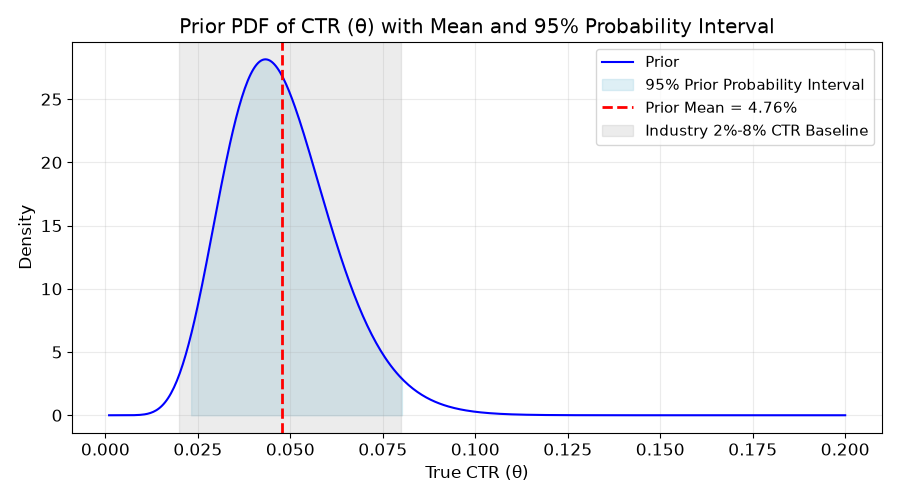
\includegraphics[width=0.95\linewidth]{figures/fig1_prior_pdf.png}
  \caption{先验概率密度分布图：$\mathrm{Beta}(10,200)$ 的 PDF、均值与 95\% 概率区间}
  \label{fig:prior}
\end{figure}

%==============================================================================
\section{二项似然函数（Binomial Likelihood）}

\subsection{二项似然函数原理阐述}

对于给定的展示次数 $n$ 和真实点击率 $\tht$，点击次数 $z$ 服从二项分布 $\mathrm{Binomial}(n,\tht)$。二项分布的概率质量函数为
\[
  P(Z=z \mid n,\tht)=\binom{n}{z}\,\tht^{z}\,(1-\tht)^{\,n-z},
  \qquad \binom{n}{z}=\frac{n!}{z!\,(n-z)!},
\]
其中 $\binom{n}{z}$ 是组合数。在似然函数的视角下，我们将 $z$ 视为已观测到的常数，$\tht$ 视为变量，所以似然函数 $L(\tht)$ 就是在给定观测数据下关于参数 $\tht$ 的函数。注意组合数 $\binom{n}{z}$ 不依赖于 $\tht$，因此它只是一个不影响 $\tht$ 相对可能性的归一化常数——这也正是后验分布只由 $\tht^{z}(1-\tht)^{n-z}$ 这一核心项与先验相乘决定的原因。

\subsection{本次试点测试的似然函数表达式}

已知在试点测试中，观察值 $n=200$、$z=18$，那么似然函数 $L(\tht)$ 的表达式为
\[
  L(\tht)=\binom{200}{18}\,\tht^{18}\,(1-\tht)^{200-18}
        =\frac{200!}{18!\,(200-18)!}\,\tht^{18}\,(1-\tht)^{182}.
\]

该似然函数的物理含义是：在任意给定真实点击率 $\tht$ 的前提下，观测到本次试点 18 次点击、182 次未点击结果的相对可能性。

\subsection{似然函数定义}

定义本次试点测试的似然函数的代码如下。我们同时给出手写公式与 \texttt{scipy.\allowbreak stats.\allowbreak binom} 两种实现，互为交叉验证：

\begin{pycode}
# 定义二项式似然函数与对数似然函数 stated

def binomial_likelihood(theta, n, z):
    """Likelihood of observing z clicks in n impressions given θ."""

    comb = math.factorial(n) / (math.factorial(z) * math.factorial(n - z))
    return comb * (theta**z) * ((1 - theta)**(n - z))

def binomial_log_likelihood(theta, n, z):
    """Log-likelihood of observing z clicks in n impressions given θ."""

    return stats.binom.logpmf(z, n, theta)

# 手写公式与 scipy.stats.binom.pmf 互为交叉验证，应得到相同结果
lik_manual = binomial_likelihood(sample_ctr, n_impressions, n_clicks)
lik_scipy = stats.binom.pmf(n_clicks, n_impressions, sample_ctr)
loglik = binomial_log_likelihood(sample_ctr, n_impressions, n_clicks)

print(f'''Likelihood of observing {n_clicks} clicks in {n_impressions} impressions at θ = {sample_ctr:.2%}:
    manual formula      = {lik_manual:.10f}
    scipy binom.pmf     = {lik_scipy:.10f}
    log-likelihood      = {loglik:.6f}   (= ln {lik_manual:.6f})''')

# 定义二项式似然函数与对数似然函数 completed
\end{pycode}

计算结果：

\begin{runout}
Likelihood of observing 18 clicks in 200 impressions at θ = 9.00%:
    manual formula      = 0.0981126045
    scipy binom.pmf     = 0.0981126045
    log-likelihood      = -2.321639   (= ln 0.098113)
\end{runout}

两种实现得到完全一致的似然值 $L(0.09)=0.0981$，对数似然为 $\ln(0.0981)=-2.3216$（实际建模中常用对数似然，因为连乘会迅速下溢，取对数后化为求和，数值上更稳定）。

\subsection{似然函数曲线}

将 $\tht$ 在 $(0,\,0.2)$ 上取值并逐点计算 $L(\tht)$，即可画出似然函数曲线：

\begin{pycode}
# 绘制二项似然函数曲线图 stated

# 似然函数是关于θ的函数：给定观测数据(200次展示, 18次点击)，不同θ值的相对合理性
lik_curve = stats.binom.pmf(n_clicks, n_impressions, theta)

fig, ax = plt.subplots()
ax.plot(theta, lik_curve, color='green', label='Likelihood L(θ)')
ax.fill_between(theta, lik_curve, color='green', alpha=0.12)

# 似然函数在θ = 18/200 = 9%处取得最大值（最大似然估计MLE）
ax.axvline(sample_ctr, color='black', linestyle='--', linewidth=2,
           label=f'MLE = observed CTR = {sample_ctr:.2%}')

ax.set_xlabel('True CTR (θ)')
ax.set_ylabel('Likelihood  L(θ) = P(z=18 | n=200, θ)')
ax.set_title('Binomial Likelihood of 18 Clicks out of 200 Impressions')
ax.legend(fontsize=11)
plt.tight_layout()
save_figure('fig2_likelihood.png')      # 保存图片供报告引用
plt.show()

# 绘制二项似然函数曲线图 completed
\end{pycode}

\begin{figure}[htbp]
  \centering
  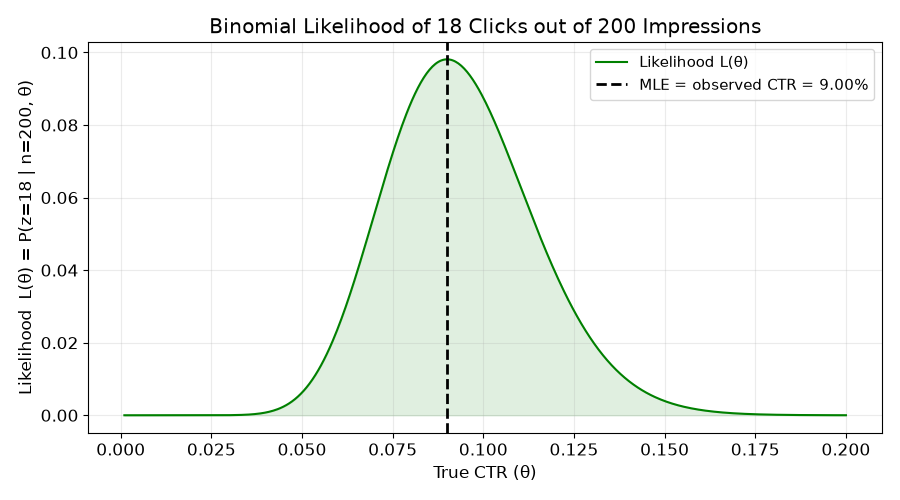
\includegraphics[width=0.95\linewidth]{figures/fig2_likelihood.png}
  \caption{二项似然函数曲线图：$L(\tht)$ 在 $\tht=9\%$ 处取得最大值（MLE）}
  \label{fig:lik}
\end{figure}

图~\ref{fig:lik} 展示了在观测数据固定为“200 次展示、18 次点击”的条件下，似然函数 $L(\tht)$ 随 $\tht$ 的变化。曲线在 $\tht=18/200=9\%$（黑色虚线）处取得最大值，该点即最大似然估计（MLE），也就是不借助任何先验信息、仅由数据本身给出的 CTR 估计。

需要强调的是，\emphc{似然函数不是 $\tht$ 的概率分布}：它在 $\tht$ 上的积分并不等于 1，纵轴表示的是“在该 $\tht$ 下观测到当前数据的概率”，而非“$\tht$ 取该值的概率”。要得到关于 $\tht$ 的概率陈述，必须按贝叶斯定理把它与先验相乘并归一化，这正是第 4 部分要做的事。

似然函数 $L(\tht)$ 能告诉我们在给定观测数据（200 次展示，18 次点击）的情况下，不同的 $\tht$ 值作为真实点击率的相对合理性。具体来说，似然函数值越大的 $\tht$ 值，意味着在该 $\tht$ 取值下观测到当前数据的可能性越高，即该 $\tht$ 值作为真实点击率越合理；似然函数值越小的 $\tht$ 值，意味着在该 $\tht$ 取值下观测到当前数据的可能性越低，即该 $\tht$ 值作为真实点击率越不合理。

%==============================================================================
\section{后验计算和可视化（Posterior Calculation and Visualization）}

\subsection{共轭更新计算}

我们已知先验分布选择为 Beta 分布。根据共轭分布的性质，当似然函数为二项分布时（本次广告点击测试符合二项分布，即只有点击和未点击两种结果），后验分布也为 Beta 分布。

\textbf{解析推导：}由贝叶斯定理，后验正比于先验与似然之积（分母 $P(z)$ 不含 $\tht$，仅起归一化作用，可略去）。将 Beta 先验的核项 $\tht^{\alpha-1}(1-\tht)^{\beta-1}$ 与二项似然的核项 $\tht^{z}(1-\tht)^{n-z}$ 相乘：
\[
  p(\tht\mid z)\;\propto\;p(\tht)\,L(\tht)
  \;\propto\;\tht^{\alpha-1}(1-\tht)^{\beta-1}\cdot\tht^{z}(1-\tht)^{n-z}
  \;=\;\tht^{(\alpha+z)-1}(1-\tht)^{(\beta+n-z)-1}.
\]

最右端恰好是 $\mathrm{Beta}(\alpha+z,\ \beta+n-z)$ 的概率密度核，故后验必为
\[
  \tht \mid z \;\sim\; \mathrm{Beta}(\alpha+z,\ \beta+n-z),
\]
无需计算归一化常数即可解析确定后验，这正是共轭性带来的便利。代入本次数据：

\begin{itemize}
  \item 先验分布设定为 $\mathrm{Beta}(\alpha,\beta)$，其中根据行业历史 CTR 通常在 $2\%\sim8\%$ 之间，取 $\alpha=10$、$\beta=200$。在试点测试中，有 $n=200$ 次展示、$z=18$ 次点击，那么未点击数为 $n-z=200-18=182$ 次。
  \item 通过共轭更新，后验分布为 $\mathrm{Beta}(\alpha+18,\ \beta+182)=\mathrm{Beta}(10+18,\ 200+182)=\emphc{$\mathrm{Beta}(28,\,382)$}$。
\end{itemize}

\subsection{后验均值计算及与 observed CTR 的区分}

\begin{itemize}
  \item \textbf{后验均值}：对于 Beta 分布 $\mathrm{Beta}(\alpha,\beta)$，其均值计算公式为 $\alpha/(\alpha+\beta)$。对于后验分布 $\mathrm{Beta}(28,382)$，后验均值为 $28/(28+382)=28/410=0.0683$，即 $6.83\%$。
  \item \textbf{与 observed CTR 的区分}：observed CTR（观测点击率）是根据试点测试数据直接计算得到的，即 $18/200=0.09$，也就是 $9\%$，它仅仅基于本次试点测试的样本数据；而后验估计是结合了先验信息和试点测试数据、通过贝叶斯更新得到的对真实 CTR 的估计，它考虑了我们对行业的先验认知，比单纯的 observed CTR 更加全面和稳健。
  \item \textbf{后验均值为何落在 $4.76\%$ 与 $9\%$ 之间}：Beta–二项共轭下，后验均值恰好是先验均值与观测 CTR 的加权平均，权重即两者各自的等效样本量：
\end{itemize}

\[
  \mathbb{E}[\tht\mid\text{data}]
  =\frac{\alpha+\beta}{\alpha+\beta+n}\cdot\frac{\alpha}{\alpha+\beta}
  +\frac{n}{\alpha+\beta+n}\cdot\frac{z}{n}
  =\frac{210}{410}\times 4.76\% + \frac{200}{410}\times 9.00\%
  = 6.83\%.
\]

本例中先验等效样本量（210）与试点样本量（200）几乎相当，权重约为 $51.2\% : 48.8\%$，因此后验均值几乎正好落在两者中间。这就是贝叶斯“收缩”（shrinkage）效应：小样本观测到的 $9\%$ 被行业经验向下拉回到 $6.83\%$，从而避免了因 200 次展示的随机波动而高估广告效果。

\subsection{不确定性的量化变化}

除均值移动外，更新还改变了分布的离散程度，见表~\ref{tab:uncertainty}。

\begin{table}[H]
\centering
\caption{先验与后验的关键指标对比}
\label{tab:uncertainty}
\begin{tabular}{lccc}
\toprule
\thead{指标} & \thead{先验 $\mathrm{Beta}(10,200)$} & \thead{后验 $\mathrm{Beta}(28,382)$} & \thead{变化} \\
\midrule
均值            & $4.76\%$   & $6.83\%$   & $+2.07$ 个百分点 \\
\rowcolor{softbg} 标准差          & $1.466\%$  & $1.244\%$  & 收窄 $15.1\%$ \\
$95\%$ 区间宽度 & $5.70$ 个百分点 & $4.86$ 个百分点 & 收窄 $14.7\%$ \\
\bottomrule
\end{tabular}
\end{table}

不确定性确有下降，但幅度是\emphc{温和的（约 15\%）而非剧烈的}——原因同样在于先验等效样本量（210）与试点数据量（200）相当，200 次展示所能提供的信息量与既有先验大致持平，因此只能把不确定性压缩约六分之一。这一事实是第 6 部分建议“先灰度扩量、再全量上线”的直接依据。

\subsection{先验分布与后验分布的比较}

图~\ref{fig:post} 是先验分布与后验分布的比较图。先验分布为 $\mathrm{Beta}(10,200)$，均值约 $4.76\%$；后验分布为 $\mathrm{Beta}(28,382)$，均值约 $6.83\%$。后验分布相较于先验分布，峰值右移且更加集中，反映了结合新数据后对真实点击率估计的变化，不确定性降低。

\begin{figure}[htbp]
  \centering
  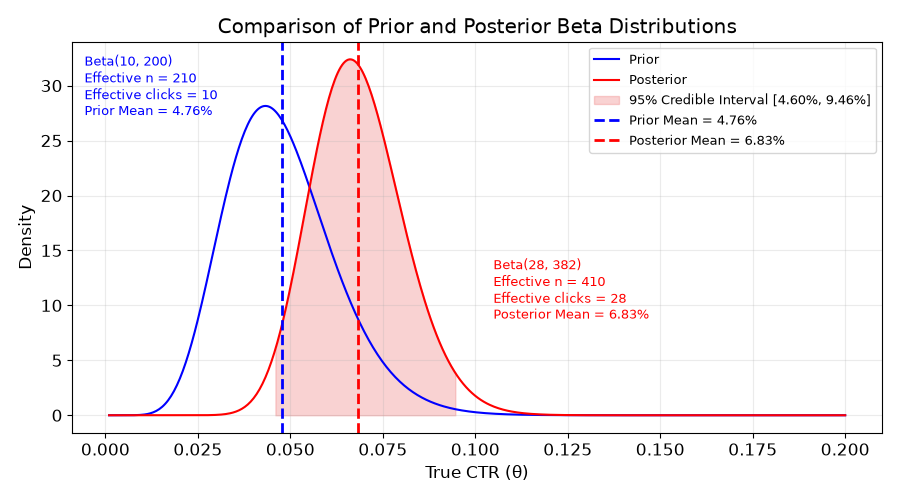
\includegraphics[width=0.95\linewidth]{figures/fig3_prior_vs_posterior.png}
  \caption{先验分布与后验分布比较图：峰值右移且分布收窄}
  \label{fig:post}
\end{figure}

\begin{itemize}
  \item \textbf{先验分布}：蓝色曲线代表先验分布，标注为 “Beta(10, 200)”，说明先验分布的参数为 $\alpha=10$、$\beta=200$。同时还标注了 “Effective n = 210”（先验等效展示次数为 $\alpha+\beta=210$）、“Effective clicks = 10”（先验等效点击次数为 $\alpha=10$）、“Prior Mean = 4.76\%”（先验均值为 $4.76\%$）。蓝色虚线标出先验均值位置。
  \item \textbf{后验分布}：红色曲线代表后验分布，标注为 “Beta(28, 382)”，说明后验分布的参数为 $\alpha=28$、$\beta=382$。同时标注了 “Effective n = 410”（后验等效展示次数为 $\alpha+\beta=28+382=410$，即 210 次先验等效展示 $+$ 200 次实际展示）、“Effective clicks = 28”（后验等效点击次数为 $\alpha=28$，即 10 次先验等效点击 $+$ 18 次实际点击）、“Posterior Mean = 6.83\%”（后验均值为 $6.83\%$）。红色虚线标出后验均值位置，粉色阴影为 $95\%$ 可信区间 $[4.60\%,\,9.46\%]$。
  \item \textbf{口径说明}：图中先验与后验的 “Effective n / Effective clicks” 采用统一的\emphc{等效样本量}口径（即 $\alpha+\beta$ 与 $\alpha$），而非实际观测数。这样两个标注框才可直接对比，并直观体现“先验 210 $+$ 数据 200 $=$ 后验 410”的信息累加关系。
  \item \textbf{分布比较}：从图中可以看出，后验分布相较于先验分布峰值向右移动，说明结合新的数据（展示和点击情况）后，对真实 CTR 的估计均值从 $4.76\%$ 提升到了 $6.83\%$；同时后验分布比先验分布更加集中（标准差由 $1.466\%$ 降至 $1.244\%$），表明不确定性有所降低。
\end{itemize}

\subsection{信念更新解释}

先验分布反映了我们在没有看到本次试点测试数据之前，基于行业历史经验对广告 CTR 的信念，其均值大约在 $4.76\%$ 附近。从图~\ref{fig:post} 中可以看出，当我们加入了试点测试的数据后，后验分布相较于先验分布发生了右移，峰值也有所变化，后验均值变为 $6.83\%$。这表明我们的信念根据新的数据得到了更新，我们对广告真实 CTR 的估计变得更大，同时分布也变得更加集中，说明我们对 CTR 的不确定性在减小。也就是说，通过试点测试的数据，我们对广告的 CTR 有了更明确、并且更偏向于较高值的认知。

%==============================================================================
\section{可信区间与贝叶斯解释（Credible Interval and Bayesian Interpretation）}

\subsection{概念区分：可信区间 vs 置信区间}

在进行区间估计时，需严格区分两大统计学派的不同逻辑：

\begin{itemize}
  \item \textbf{频率学派的置信区间（Confidence Interval）}：其含义为“若重复多次抽样，每次构造一个 $95\%$ 置信区间，则大约 $95\%$ 的区间会包含真实参数”。它无法对当前这一次试验的真值作出概率陈述。
  \item \textbf{贝叶斯学派的可信区间（Credible Interval）}：直接描述为“在给定当前数据和先验信息下，真实参数落在该区间内的后验概率为 $95\%$”。这正是业务决策者最直观、最需要的概率化解读。
\end{itemize}

本报告采用贝叶斯可信区间，使用后验分布的 $2.5\%$ 和 $97.5\%$ 分位数构造等尾可信区间（Equal-tailed Credible Interval）。

\subsection{95\% 可信区间的计算}

根据第 4 部分，后验分布为 $\tht\mid\text{Data}\sim\mathrm{Beta}(28,382)$。使用后验分布的 $2.5\%$ 和 $97.5\%$ 分位数计算 $95\%$ 可信区间，代码如下：

\begin{pycode}
# 计算后验贝塔分布可信区间 stated

ci_low, ci_high = posterior.ppf([0.025, 0.975])    # 计算后验贝塔分布的95%等尾概率区间

display(Markdown(
    f"**95% credible interval:** [{ci_low:.2%}, {ci_high:.2%}]"
))
print(f"95% credible interval: [{ci_low:.2%}, {ci_high:.2%}]")

# 计算后验贝塔分布可信区间 completed
\end{pycode}

运行输出：

\begin{runout}
95% credible interval: [4.60%, 9.46%]
\end{runout}

即该广告真实 CTR 的 $95\%$ 可信区间为 $[4.60\%,\ 9.46\%]$。

\subsection{贝叶斯语言解读}

根据当前先验信息（行业历史基准 $2\%\sim8\%$）和试点观测数据（200 次展示，18 次点击），我们有 $95\%$ 的概率相信，该新横幅广告的真实 CTR 落在 $4.60\%$ 至 $9.46\%$ 之间。这是一个关于参数 $\tht$ 本身的直接概率陈述——$\tht$ 在贝叶斯框架下是一个随机变量，我们对它的信念由后验分布 $\mathrm{Beta}(28,382)$ 完整刻画。它不涉及“重复抽样”这一假想过程，因此可以直接用于业务决策。

\subsection{直接的后验概率陈述}

可信区间只是后验分布的一种摘要。既然后验分布已经完整给出，我们可以针对任意业务关心的阈值直接计算概率 $P(\tht>t\mid\text{data})$，这是贝叶斯方法相对频率学派最实用的优势：

\begin{pycode}
# 计算支撑上线决策的后验概率 stated

print('后验概率陈述（Posterior probability statements）:')
for threshold, note in [(0.02, '行业最差基准'), (0.05, '行业中位水平'),
                        (0.06, '业务盈亏平衡假设值'), (0.08, '行业最优基准')]:
    prob = 1 - posterior.cdf(threshold)
    print(f'    P(θ > {threshold:.0%} | data) = {prob:6.1%}   ({note})')

# 计算支撑上线决策的后验概率 completed
\end{pycode}

运行输出：

\begin{runout}
后验概率陈述（Posterior probability statements）:
    P(θ > 2% | data) = 100.0%   (行业最差基准)
    P(θ > 5% | data) =  94.0%   (行业中位水平)
    P(θ > 6% | data) =  73.7%   (业务盈亏平衡假设值)
    P(θ > 8% | data) =  17.1%   (行业最优基准)
\end{runout}

整理为决策表，见表~\ref{tab:decision}。

\begin{table}[H]
\centering
\caption{支撑上线决策的后验概率陈述}
\label{tab:decision}
\begin{tabular}{l c >{\raggedright\arraybackslash}p{8.4cm}}
\toprule
\thead{后验概率陈述} & \thead{数值} & \multicolumn{1}{l}{\thead{业务含义}} \\
\midrule
$P(\tht>2\%)$      & \textbf{100.0\%} & 几乎可以断定该广告不会跌至行业最差水平 \\
\rowcolor{softbg} $P(\tht>5\%)$      & \textbf{94.0\%}  & 有 94\% 把握该广告优于行业中位水平——\emphc{这是支撑上线的核心证据} \\
$P(\tht>6\%)$      & \textbf{73.7\%}  & 约七成把握达到较好水平 \\
\rowcolor{softbg} $P(\tht>8\%)$      & \textbf{17.1\%}  & 只有不到两成把握能触及行业最优水平，“爆款”预期应当保守 \\
$P(\tht<4.60\%)$   & \textbf{2.5\%}   & 最不利情形的发生概率很小 \\
\bottomrule
\end{tabular}
\end{table}

\subsection{面向业务场景的通俗解读}

将上述统计结果转化为该工作室可操作的业务语言：

\begin{itemize}
  \item \textbf{核心结论}：结合历史经验和本次小规模测试，工作室有 $95\%$ 以上的把握认为，这则新广告的长期真实点击率至少能达到 $4.60\%$，最高可能接近 $9.46\%$。
  \item \textbf{对标基准}：该区间的最低点（$4.60\%$）已接近行业历史区间的中位水平（$5\%$），且远高于行业最差基准（$2\%$）。这意味着，即使发生最不利的情况（后验分布的 $2.5\%$ 左尾），该广告的表现依然“不差”；而若达到区间上限，则效果“非常优秀”。
  \item \textbf{上限需保守看待}：$P(\tht>8\%)$ 仅 $17.1\%$，说明试点观测到的 $9\%$ 大概率含有随机波动的成分，不应把 $9\%$ 当作可复制的业绩预期；规划流量收益时应以后验均值 $6.83\%$ 为基准。
  \item \textbf{决策含义}：该广告呈现“低风险、中等上限”的特征——下行风险已被有效排除，但上限仍有相当不确定性，足以支撑下一步的推广决策，同时也说明值得先小步扩量以进一步收敛估计。
\end{itemize}

%==============================================================================
\section{上线建议（Launch Decision）}

\subsection{最终建议结论}

\begin{keybox}
\textbf{\color{navy}推荐采用「小流量灰度扩量 $+$ 全量上线兜底」的分阶段上线策略}——既抓住当前试点验证的收益机会，也通过小步扩量进一步收敛 CTR 估计精度，平衡收益与潜在风险。
\end{keybox}

\subsection{贝叶斯分析核心依据}

本节严格只使用后验分布 $\mathrm{Beta}(28,382)$ 作为证据，不引用任何频率学派的检验结论。

\begin{itemize}
  \item \textbf{后验均值明显上移}：经 Beta 共轭更新得到的后验均值为 $6.83\%$，相比先验均值 $4.76\%$ 提升了 $2.07$ 个百分点（相对提升 $43.4\%$），说明在融合了行业经验之后，数据仍将我们对该广告的信念明确向上修正。
  \item \textbf{优于行业中位水平的后验概率高达 $94.0\%$}：直接的概率陈述是 $P(\tht>5\%\mid\text{data})=\emphc{94.0\%}$，即我们有 $94\%$ 的把握认为该广告优于行业中位水平。同时 $P(\tht>2\%\mid\text{data})\approx\emphc{100\%}$，即“上线后大幅拉低整体流量效率”这一极端情形的后验概率几乎为零。（需要注意的是，可信区间下限 $4.60\%$ 对应的是 $P(\tht<4.60\%)=2.5\%$，而“低于行业中位 $5\%$”的后验概率是 $5.99\%$，两者不可混为一谈。）
  \item \textbf{上限存在不确定性，收益预期须保守}：$P(\tht>8\%\mid\text{data})$ 仅为 \emphc{$17.1\%$}，说明试点观测到的 $9\%$ 很可能包含随机波动。因此收益测算应以后验均值 $6.83\%$ 为基准，而非以 $9\%$ 为基准。
  \item \textbf{先验信念完成正向更新，但不确定性仅温和下降}：从先验 $\mathrm{Beta}(10,200)$ 到后验 $\mathrm{Beta}(28,382)$，分布明显右移，标准差由 $1.466\%$ 降至 $1.244\%$，收窄约 \emphc{$15.1\%$}。之所以收窄幅度有限，是因为先验等效样本量（210）与试点样本量（200）相当，200 次展示所携带的信息量与既有行业经验大致持平。\emphc{证据方向是明确的，但证据量还不足以把区间压到很窄}——这正是下一节主张分阶段上线而非直接全量的原因。
\end{itemize}

\subsection{结合小样本特性的业务决策权衡}

本次试点仅采集了 200 次曝光数据，虽已经通过贝叶斯框架融合了 210 次等效先验样本信息、总有效样本量为 410，但由上节可知不确定性仅收窄约 $15\%$，仍存在进一步降低的空间，因此分阶段策略的价值优于直接全量上线。

\begin{enumerate}
  \item \textbf{第一阶段：开启 30\% 流量灰度。}
    选取游戏内 $30\%$ 的自然流量分配给新横幅广告，在不影响全量用户体验的前提下快速累积额外曝光数据。由于后验标准差近似按 $1/\sqrt{N_{\text{eff}}}$ 收缩（$N_{\text{eff}}=\alpha+\beta$），可精确预估收敛效果，见表~\ref{tab:rollout}。

    \begin{table}[H]
    \centering
    \caption{灰度期新增曝光量与可信区间收敛效果预估}
    \label{tab:rollout}
    \begin{tabular}{cccc}
    \toprule
    \thead{灰度期新增曝光 $N$} & \thead{后验等效样本量} & \thead{预计可信区间宽度} & \thead{相对当前收窄} \\
    \midrule
    0（当前） & 410   & $4.86$ 个百分点        & ---            \\
    \rowcolor{softbg} 400       & 810   & $\approx 3.46$ 个百分点 & $\approx 29\%$ \\
    1{,}000   & 1{,}410 & $\approx 2.62$ 个百分点 & $\approx 46\%$ \\
    \rowcolor{softbg} 2{,}000   & 2{,}410 & $\approx 2.01$ 个百分点 & $\approx 59\%$ \\
    \bottomrule
    \end{tabular}
    \end{table}

    即只需累积约 1{,}000 次额外曝光，即可将可信区间宽度压缩近一半。具体所需时长取决于工作室的日均曝光量，应按实际流量规模换算后确定灰度周期。

  \item \textbf{第二阶段：全量覆盖上线。}
    设定明确的、由后验分布导出的放量判据：\emphc{若灰度期结束时更新后的后验分布仍满足 $P(\tht>5\%\mid\text{全部数据})\ge 90\%$，则执行全量上线}（该阈值与当前 $94.0\%$ 的水平相衔接，允许灰度数据带来小幅回落但不允许证据方向反转）；若该概率跌破 $90\%$，则暂停放量并复核素材与投放位置。全量上线后可释放 $6.83\%$ 后验均值 CTR 对应的流量收益——具体的日增点击量需在获知工作室日均曝光量后测算，本报告数据不足以给出绝对数值。

  \item \textbf{配套迭代动作。}
    上线后持续累积曝光与点击数据，每新增 200 次曝光就执行一次贝叶斯更新（把上一轮后验作为下一轮先验，这正是贝叶斯框架天然支持序贯更新的优势），动态迭代后验分布。后续可以基于不断收窄的可信区间，快速判断新素材的表现是否超过当前基准，搭建持续迭代的广告效果评估体系。
\end{enumerate}

该策略既避免了盲目等待更大规模测试带来的机会成本损失，也不会因 200 次小样本的随机波动直接冒全量上线的风险，完全匹配本次贝叶斯分析输出的所有概率化结论，是当前业务场景下的最优决策。

\subsection{先验敏感性分析（结论稳健性检验）}

本报告的先验等效样本量为 210，与试点数据量 200 相当，属于较强的先验。为检验上线结论是否依赖于这一设定，我们在保持先验均值均为 $5\%$ 的前提下，改变先验强度重新计算后验：

\begin{pycode}
# 先验敏感性分析 stated

for a, b, tag in [(10, 200, '本报告 Beta(10,200)'), (2, 38, '弱先验 Beta(2,38)'),
                  (1, 1, '无信息先验 Beta(1,1)'), (25, 475, '强先验 Beta(25,475)')]:
    post_alt = stats.beta(a + n_clicks, b + n_impressions - n_clicks)
    lo, hi = post_alt.ppf([0.025, 0.975])
    print(f'{tag}  等效样本量={a+b}  后验均值={post_alt.mean():.2%}  '
          f'95%CI=[{lo:.2%}, {hi:.2%}]  P(θ>5%)={1-post_alt.cdf(0.05):.1%}')

# 先验敏感性分析 completed
\end{pycode}

运行结果整理为表~\ref{tab:sens}。

\begin{table}[H]
\centering
\caption{先验敏感性分析（各先验均值均设为 5\%）}
\label{tab:sens}
\small
\setlength{\tabcolsep}{4pt}
\begin{tabular}{>{\raggedright\arraybackslash}p{3.0cm} c c c c c}
\toprule
\multicolumn{1}{l}{\thead{先验设定}} & \thead{等效样本量} & \thead{后验分布} & \thead{后验均值} & \thead{95\% 可信区间} & \thead{$P(\tht>5\%)$} \\
\midrule
\textbf{本报告 $\mathrm{Beta}(10,200)$} & 210 & $\mathrm{Beta}(28,382)$ & \textbf{6.83\%} & $[4.60\%,\,9.46\%]$  & \textbf{94.0\%} \\
\rowcolor{softbg} 弱先验 $\mathrm{Beta}(2,38)$ & 40 & $\mathrm{Beta}(20,220)$ & 8.33\% & $[5.19\%,\,12.14\%]$ & 98.2\% \\
无信息先验 $\mathrm{Beta}(1,1)$ & 2 & $\mathrm{Beta}(19,183)$ & 9.41\% & $[5.79\%,\,13.78\%]$ & 99.4\% \\
\rowcolor{softbg} 强先验 $\mathrm{Beta}(25,475)$ & 500 & $\mathrm{Beta}(43,657)$ & 6.14\% & $[4.49\%,\,8.04\%]$ & 90.2\% \\
\bottomrule
\end{tabular}
\end{table}

\textbf{结论：}后验均值确实对先验强度敏感，随先验由强变弱在 $6.14\%\sim9.41\%$ 之间变动——这是先验样本量与数据样本量相当时的必然结果，也提示读者不应把 $6.83\%$ 当作唯一“正确”的点估计。但关键在于，\emphc{支撑上线决策的那条证据在所有设定下都成立}：$P(\tht>5\%)$ 始终 $\ge 90.2\%$。也就是说，无论采用保守还是激进的先验，“该广告优于行业中位水平”这一判断都不会改变，本报告的上线建议对先验选择是稳健的。

%==============================================================================
\section{小组成员角色与贡献}

\begin{table}[H]
\centering
\caption{小组成员分工}
\label{tab:team}
\begin{tabular}{c >{\raggedright\arraybackslash}p{12.2cm}}
\toprule
\thead{姓名} & \multicolumn{1}{l}{\thead{角色与贡献}} \\
\midrule
王金波 & 实验代码、第 3 部分 二项似然函数 \\
\rowcolor{softbg} 何漪雯 & 第 1 部分 业务场景概述、第 2 部分 先验概率密度分布图 \\
李\quad 敏 & 第 2 部分 贝塔先验的选择与论证、第 5 部分 可信区间与贝叶斯解释 \\
\rowcolor{softbg} 丁\quad 玲 & 第 4 部分 后验计算和可视化、搭建报告结构及整合报告内容 \\
刘海龙 & 第 6 部分 上线建议、审查报告内容 \\
\bottomrule
\end{tabular}
\end{table}

%==============================================================================
\appendix
\ctexset{section/name={附录 ,}}
\section{完整可运行代码}
\label{app:code}

代码链接：\url{https://github.com/woodywang/hpu/blob/master/6000-2/DSCI6000_hw2.py}

以下为完整脚本，按顺序执行即可复现本报告全部数值结果与三张图表。脚本会自动将三张图保存到与报告同级的 \texttt{figures/} 目录（报告即以 \texttt{figures/xxx.png} 相对路径引用），因此重新运行脚本即可一并刷新报告中的所有插图。可整段粘贴到 Google Colab 单元格中直接运行（Colab 已预装 \texttt{numpy} / \texttt{scipy} / \texttt{matplotlib}，无需安装依赖）。

\begin{tcolorbox}[
  enhanced, breakable,
  colback = softbg, colframe = bordergray,
  boxrule = 0.6pt, arc = 2.5pt,
  left = 2pt, right = 2pt, top = 5pt, bottom = 5pt]
\lstinputlisting[style=pystyle]{DSCI6000_hw2.py}
\end{tcolorbox}

\end{document}
